\documentclass[11pt]{article}
\usepackage[T1]{fontenc}
\usepackage[utf8]{inputenc}
\usepackage{lmodern,microtype}
\usepackage[margin=1in]{geometry}
\usepackage{amsmath,amssymb,amsthm,mathtools}
\usepackage{booktabs,tabularx,array,longtable}
\usepackage{xcolor,enumitem,fancyhdr,lastpage,listings}
\usepackage{tikz}
\usetikzlibrary{arrows.meta,positioning}
\usepackage[breaklinks=true,colorlinks=true,linkcolor=blue!45!black,urlcolor=blue!50!black,citecolor=blue!45!black]{hyperref}
\usepackage{bookmark}
\definecolor{ink}{HTML}{17324D}
\definecolor{teal}{HTML}{006D77}
\definecolor{pale}{HTML}{F1F5F8}
\pagestyle{fancy}
\fancyhf{}
\fancyhead[L]{\small\textcolor{ink}{K215: proof fusion and local reuse}}
\fancyhead[R]{\small Research proposal}
\fancyfoot[C]{\small\thepage\ / \pageref{LastPage}}
\setlength{\headheight}{14pt}
\setlength{\parindent}{0pt}
\setlength{\parskip}{5pt plus 1pt}
\setlength{\emergencystretch}{3em}
\setlist{itemsep=3pt,topsep=4pt,leftmargin=*}
\newtheorem{theorem}{Theorem}[section]
\newtheorem{lemma}[theorem]{Lemma}
\newtheorem{proposition}[theorem]{Proposition}
\theoremstyle{definition}\newtheorem{definition}[theorem]{Definition}
\newcommand{\Con}{\operatorname{Con}}
\newcommand{\Halt}{\operatorname{Halt}}
\newcommand{\Comp}{\operatorname{Compilable}}
\newcommand{\Exec}{\operatorname{Exec}}
\newcommand{\ctr}{\operatorname{Contract}}
\newcommand{\Reads}{\operatorname{Reads}}
\newcommand{\Ready}{\operatorname{Ready}}
\newcommand{\code}[1]{\texttt{#1}}
\newcommand{\pin}{6d9800d1ca67c52db0eb6e1c65df7b5cab9cdb95}
\newcommand{\repo}{https://github.com/VladimirReshetnikov/ProveIt/blob/6d9800d1ca67c52db0eb6e1c65df7b5cab9cdb95/}
\lstset{basicstyle=\ttfamily\small,columns=fullflexible,keepspaces=true,
  breaklines=true,frame=single,rulecolor=\color{black!18},backgroundcolor=\color{pale},
  xleftmargin=4pt,xrightmargin=4pt,aboveskip=8pt,belowskip=8pt}
\hypersetup{pdftitle={K215 Proof Fusion and Local Reuse},pdfauthor={Research contribution for the ProveIt project}}

\begin{document}
\begin{titlepage}
\vspace*{0.5cm}
{\color{teal}\large PROVEIT / BUSY BEAVER RESEARCH}\par
\vspace{0.8cm}
{\color{ink}\Huge\bfseries Shortening the K215\par correctness proofs}\par
\vspace{0.45cm}
{\LARGE Direct compilation into contracts\par and certified local proof reuse}\par
\vspace{0.9cm}
{\large October 21, 2026 (Pacific time)}\par
\vspace{0.5cm}
\textbf{Repository baseline}\par
\href{\repo}{VladimirReshetnikov/ProveIt}, revision\par
{\small\ttfamily\pin}\par
\vspace{0.8cm}
\begin{abstract}
The maintained K215 proof has already undergone fourteen Lean simplification
phases. We identify a further structural reduction and implement it in both
proof languages: interpret the existing dominated-implication theorem in the
predicate ``has a finite program satisfying the block contract.'' This compiles
the original numerical calculus directly and removes its intermediate dominated
calculus from the compiler dependency path. The Lean and Rocq-family components
are checked, with preserved public enumerator/seed interfaces and explicit
compatibility adapters.

A second contribution completes an earlier dependency-transport proposal for
the actual Lean symbolic interpreter, including the maintained Home shortcut.
Agreement on a saved finite set of table queries transports the exact executor
result; target register semantics and halting conditions remain separate.
An independent finite replay of all 6,176 K215 outcomes measures the local
supports and records reproducible evidence. We distinguish these new checks
from existing production endpoint receipts and give a prioritized integration
plan for both proof assistants.
\end{abstract}
\vfill
\colorbox{pale}{\parbox{0.94\textwidth}{\textbf{Status.} Checked proof components and
reviewable patches. The full modified physical-machine-to-ZFC endpoints have
not been rebuilt. The machine table, state count, numerical semantics and final
claimed equivalence are not changed by the compiler patches.}}
\end{titlepage}
\setcounter{page}{2}

{\small\setlength{\parskip}{0pt}\tableofcontents}
\newpage

\section{Recommendation and deliverable}

The best immediate simplification is to \textbf{compile directly in the algebra
of block contracts}. The current compiler first translates a derivation of
\code{C222} (Rocq: \code{thm222}) into a dominated calculus and then compiles that
second derivation. The existing generic implication theorem is already strong
enough to eliminate the intermediate derivation. Its predicate parameter can be
the compiler's own semantic specification.

This is a modest source reduction with a useful conceptual effect: one inductive
calculus, one translation induction and one equivalence interface disappear from
the active compiler dependency path. We supply actual Lean and Rocq-family
patches rather than only an architectural suggestion. A second, independent
component proves when the maintained symbolic checks can be reused after a
table change. It resolves the interpreter-local obligation left open in the
earlier \code{rocq-composition} proposal~\cite{priortransport}.

The archive contains this article and its LaTeX source; the compiler patches,
overlays and compatibility clients; the new Lean transport library and audit
client; compiler receipts and logs; a finite Python replay of all current site
outcomes; exact input tables and source-site data; and reproduction instructions.
All empirical quantities below are either source counts or named check results.
We do not infer kernel time reductions from byte counts or query counts.

\begin{table}[h]
\centering\small
\begin{tabularx}{\textwidth}{@{}p{0.23\textwidth}X p{0.26\textwidth}@{}}
\toprule
Contribution & Result supplied & Verification boundary\\
\midrule
Direct Lean compiler & \code{build\_c222}; dominated API moved to an optional import & Lean 4.32.0; focused fresh build and typed clients\\
Direct Rocq compiler & \code{compile\_direct}; templates and generated copies synchronized & Coq 8.18.0; six closed client reports and recursive \code{coqchk}\\
Runtime dependency transport & Production-step locality, exact executor transfer, saved-support interface & Lean 4.32.0; six fresh dependencies, library and client\\
K215 footprint census & All 4,751 leaves and 6,176 guarded outcomes replay successfully & Independent Python audit; not a kernel certificate\\
\bottomrule
\end{tabularx}
\end{table}

\section{Baseline: what has already been simplified}

The baseline is the exact revision on the title page, not an earlier 215-state
snapshot. The repository's phase-fourteen record reports a 178-module Lean
endpoint selecting 2,093,112 bytes of project source. It already shares derived
rules between the named calculi and proves profile contracts under transitive
containers~\cite{phase14}. Our independent static import census reproduces that
178-module, 2,093,112-byte baseline and counts 40,517 physical source lines.

Several tempting suggestions would therefore repeat work already done:
\begin{itemize}
\item \code{KEndpoint215} is already a short instance of a generic endpoint
composition theorem. Its 54 lines are not the principal source of complexity.
\item Lean already uses one forward normalized source certificate, with 1,426
entries, balanced lookup and the corresponding generic equivalence theorem.
Recommending elimination of a mirrored Lean certificate would be obsolete.
\item \code{L2AxiomsPerm} already represents the AX routine by a checked word
of register macros, composes its contracts by one induction and identifies the
result with the enumerator's abstract AX operation.
\item \code{EnumPerm.halts\_iff} already works from arbitrary states between
candidates satisfying the derivability invariant. The seed is already an
instance of this theorem.
\item The generic implication core, its numerical adapter and the shared Home
return shortcut are already maintained. The new work uses them.
\end{itemize}
These facts are directly visible in the maintained sources and checkpoint
record~\cite{endpoint,enum,axioms,phase14}.

The two proof languages are at different integration stages. Rocq production
still uses the two-direction 2,240-entry source certificate and the older
reflective dominated-implication implementation. Earlier packets contain checked
normalized, balanced and shorter implication components, but their existence is
not a production acceptance result for the current full endpoint~\cite{rocqsource,priorindex}.

\subsection{The endpoint that must be preserved}

The maintained Lean statement is
\begin{lstlisting}
KEndpoint215.blank_halts_iff_zfc_refutation :
  BlankHalts machine215 <-> BProv ZFCax_s [] Form.fBot
\end{lstlisting}
with its nonhalting companion obtained by negation. The Rocq dense endpoint is
\begin{lstlisting}
K215F.CorrectDense215.tm215_halts_iff_ZFC_inconsistent
\end{lstlisting}
The repository records completed checks for the original production sources in
both languages~\cite{candidate,rocqverify}. Those historical receipts remain
receipts for their exact original source bytes.

The intended mathematical equivalence remains
\[
  \neg\Halt(M_{215},\mathrm{blank})\quad\longleftrightarrow\quad\Con(\mathrm{ZFC}).
\]
The present contribution refactors the external formal correctness chain. It
does not establish a new internal PA endpoint or supply a new formal
arithmetization of this entire chain inside ZFC. The repository itself separates
those tasks. No assumption of \(\Con(\mathrm{ZFC})\) is used to simplify the
halting equivalence.

\section{Direct compilation into the contract predicate}
\label{sec:fusion}

\subsection{The existing contract is already the right abstraction}

For a finite command list \(p\) and formula code \(x\), the Lean contract is
exactly
\begin{align}
\ctr(p,x)\;\equiv\;\forall T,S,\quad
 &\operatorname{cexec}(p,\langle T,S,0,0\rangle)=\mathrm{none}\nonumber\\[-2pt]
 &\quad\lor\quad
 \operatorname{cexec}(p,\langle T,S,0,0\rangle)
   =\mathrm{some}\langle x,S,0,0\rangle.
\label{eq:contract}
\end{align}
The Rocq predicate \code{blk X L} has the same purpose. It is essential to retain
both disjuncts. The interpreter may discover the falsity code while executing a
subprogram; the correct compiler contract permits that early halt. Requiring
every block to return normally would invalidate existing composition lemmas.

Define
\[
  \Comp(x)\;\equiv\;\exists p\in\operatorname{List}(\mathrm{Cmd}),\ \ctr(p,x).
\]
The witness \(p\) precedes the universal quantifiers over \(T,S\). Thus a single
finite list works uniformly for every initial formula and stack. A statement
\(\forall T,S\,\exists p\) would be too weak for the enumerator completeness
argument. This quantifier order is unchanged by our implementation.

\subsection{Use the general implication theorem at this predicate}

Write \(I(a,b)\) for the numerical implication constructor \code{wim}. The
repository's numerical \(\rho_8\) theorem is uniform in a predicate
\(P:\mathbb N\to\mathrm{Prop}\). In the maintained Lean interface, its
assumptions are
\begin{align*}
 &P(I(a,b))\ \land\ P(a)\ \Longrightarrow\ P(b),\\
 &u\le a\ \Longrightarrow\ P(\rho_8(a,b,c,u)).
\end{align*}
Its conclusion is \(P(\rho_8(a,b,c,u))\) for arbitrary \(a,b,c,u\), without the
order restriction. This is \code{DomRho8.rho8\_all\_of\_restricted}~\cite{domrho}.
The maintained Rocq \code{DomImp} interface also requests truth; the existing
\code{blk\_true} discharges that extra field.

Now take \(P=\Comp\). The required premises are already implemented:
\begin{enumerate}
\item Given witnesses for \(\Comp(a)\) and \(\Comp(I(a,b))\), combine their
programs with \code{mpBlock} (Rocq: \code{mpb}). The existing
\code{mp\_contract}/\code{blk\_mp} proves the result.
\item When \(u\le a\), the current AX leaf implementation supplies a uniform
block for \(\rho_8(a,b,c,u)\). The guard justifies the subtraction \(a-u\)
in the generated command parameters.
\item In Rocq, the existing discard block supplies truth.
\end{enumerate}

\begin{theorem}[Compiler fusion]
Every \code{C222} derivation of a code \(x\) has a finite block satisfying
\(\ctr(p,x)\), without constructing an intermediate \code{CDom} derivation.
\end{theorem}
\begin{proof}
First apply the generic dominated-implication theorem with predicate
\(\Comp\), using the two closures just established. This gives a block for
every unrestricted \(\rho_8\) instance. Induct on the original \code{C222}
derivation. Its truth, modus-ponens, generalization, other row and gated-bundle
cases use the unchanged existing compiler operations. Its unrestricted
\(\rho_8\) case uses the result of the first step. Every constructor therefore
produces an existential witness for the same uniform contract.
\end{proof}

The proof is an instance of induction into a predicate closed under the rules.
Its value here is that the predicate is the semantic correctness specification
of an actual program. No new axiomatization, interpretation of formula codes or
formula-decoding invariant is needed.

\begin{center}
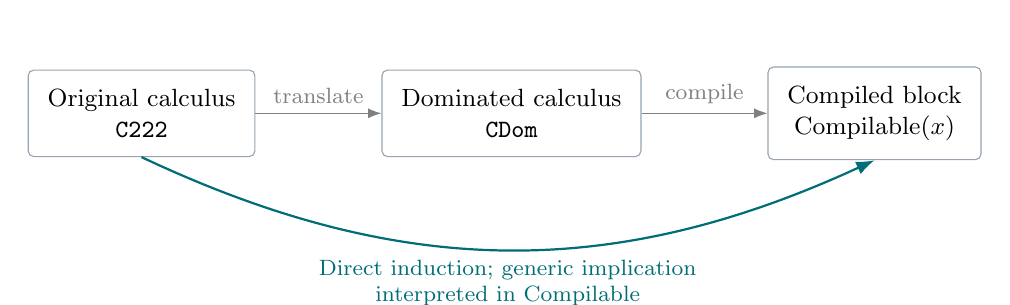
\begin{tikzpicture}[node distance=9mm and 16mm,>=Latex,
  box/.style={draw=ink!45,rounded corners=2pt,align=center,inner sep=7pt,font=\small}]
\node[box] (c) {Original calculus\\\code{C222}};
\node[box,right=of c] (d) {Dominated calculus\\\code{CDom}};
\node[box,right=of d] (p) {Compiled block\\\(\Comp(x)\)};
\draw[->,black!50] (c)--node[above,font=\footnotesize]{translate}(d);
\draw[->,black!50] (d)--node[above,font=\footnotesize]{compile}(p);
\draw[->,teal,thick] (c.south) to[bend right=25]
  node[below,align=center,font=\footnotesize]{Direct induction; generic implication\\interpreted in \(\Comp\)} (p.south);
\end{tikzpicture}
\end{center}

\subsection{Implementation in Lean}

The modified \code{EnumPerm} imports \code{KCode222} and \code{DomRho8}
directly. Its new theorem is
\begin{lstlisting}
theorem build_c222 :
  C222 n -> exists p : List Cmd, Contract p n
\end{lstlisting}
and the substantive unrestricted-row case is
\begin{lstlisting}
DomRho8.rho8_all_of_restricted
  (T := fun n => exists p : List Cmd, Contract p n)
  hmp hrow a b c u
\end{lstlisting}
The completeness theorem calls \code{build\_c222 h} directly, replacing
\code{build (cdom\_of\_c222 h)}. The executable definitions and public
\code{sound}, \code{complete} and \code{halts\_iff} signatures remain unchanged.

The previous \code{EnumPerm.build} interface remains available through the
optional \code{EnumPermCompat} import. The adapter converts its dominated
premise back to \code{C222} and invokes the direct compiler. This is an explicit
import migration for clients using the old internal compiler theorem; it is
not a claim of complete import-transparent compatibility. Keeping the old
dominated theorem in the active module would retain the dependency we want to
remove. \code{KCodeDom} remains available for the older machine and standalone
calculus developments.

\subsection{Implementation in Rocq}

The implementation constructs \code{DomImp Compilable} from
\code{blk\_true}, \code{blk\_mp} and \code{blk\_r8}. Its new theorem is
\begin{lstlisting}
compile_direct :
  forall X, thm222 X -> exists L, blk X L.
\end{lstlisting}
Both \code{enum\_complete} and \code{seedPerm\_complete} use it directly.
A separate module preserves the old dominated compiler statement as
\code{CompilerDomCompat.compile}. The old fully qualified
\code{L1\_CompPerm.compile} name is intentionally replaced; public seed and
enumerator types are checked unchanged.

The patch updates the two \code{rocqperm} templates and their generated
\code{K215F} copies together. It updates the two affected source hashes in the
extension manifest and preserves the existing source-header hashing and
namespace substitution. The generation mechanism remains unchanged. A source
audit checks these bindings and successful patch application to the pin.

\section{Measured effect and fresh verification}

\subsection{Source reductions: count the right objects}

\begin{table}[h]
\centering\small
\begin{tabular}{@{}lrrr@{}}
\toprule
Selected dependency closure & Baseline & Proposed & Change\\
\midrule
Lean endpoint modules & 178 & 177 & $-1$\\
Lean endpoint source lines & 40,517 & 40,452 & $-65$\\
Lean endpoint source bytes & 2,093,112 & 2,091,052 & $-2,060$\\
Rocq K215F modules & 42 & 41 & $-1$\\
Rocq K215F source lines & 9,939 & 9,880 & $-59$\\
Rocq K215F source bytes & 1,821,394 & 1,819,829 & $-1,565$\\
\bottomrule
\end{tabular}
\caption{Static source-closure counts for the compiler fusion alone. These are
not measurements of rebuilt complete endpoints. Physical lines include comments
and blanks; compatibility modules are outside the selected endpoint closure.}
\end{table}

The Lean compiler file itself grows from 545 to 553 lines, while the 73-line
\code{KCodeDom} leaves the active closure. Hence the net reduction is 65 lines.
Its new optional compatibility module has 16 lines and 581 bytes. The Rocq
compiler grows by 11 lines and 376 bytes; the seed loses 21 bytes; the 70-line,
1,920-byte \code{ThmDom} dependency leaves the closure. Hence its net reduction
is 59 lines and 1,565 bytes.

These are reductions of the source selected to justify the endpoint. Total
repository storage grows because legacy calculus files are retained and
compatibility adapters are added. The corresponding full Rocq closure is
predicted to fall from 237 to 236 sources if its 195 reference modules remain
the same. We have freshly audited the 42-to-41 K215F portion; we have not rebuilt
the full 236-source endpoint.

The 176-line runtime library in Section~\ref{sec:reuse} is an independent new
component, with a separate 63-line audit client. It is not silently included in,
or subtracted from, the compiler-only savings above. Its purpose is to simplify
future proof reuse; adding it increases library source size.

\subsection{What was compiled}

The Lean compiler run freshly compiled 16 project modules and two explicit
audit clients, including the optional compatibility path. It then rebuilt the
original \code{EnumPerm} and a baseline audit using only the byte-identical
dependency objects from the first run. The original and new compiler,
completeness and halting-interface reports have exactly
\code{propext}, \code{Classical.choice} and \code{Quot.sound}. The proposed
source and audit clients have no warnings. Six preexisting warnings occur in
the unchanged \code{TarskiComplete} dependency.

The Rocq-family run used Coq 8.18.0 and OCaml 4.14.1. It compiled 11
project/calculus modules and a typed client. All six client assumption reports
are closed under the global context, and recursive \code{coqchk} passed for
the seed theorem, compatibility module and client. Private compilation copies
replace the \code{Stdlib} import prefix by \code{Coq} where required by this
toolchain; the receipt binds both original and compiled bytes. The maintained
1,169-line \code{DomRho8.v} is unchanged, so this experiment isolates the
compiler fusion from earlier implication-shortening work.

This is not the designated production Rocq 9.1.0/stdlib 9.0.0 acceptance run.
Nor did we rebuild the complete modified Lean physical endpoint. The focused
checks establish the changed component theorems and selected unchanged public
interfaces. Production acceptance must recompile affected descendants and
the exact closed endpoint clients, with fresh source/object provenance.

\section{Reuse symbolic checks by their actual dependencies}
\label{sec:reuse}

Compiler fusion removes a logical intermediate object. The remaining large
computational burden is different: many site checks execute similar paths
through the same table. To make future variations easier to verify, a proof
should expose which rows of the table it actually depends on.

The earlier dependency proposal gave a generic trace idea and left its
interpreter-locality obligation open~\cite{priortransport}. Our new
\code{KRuntimeDependency.lean} proves that obligation for the exact maintained
\code{KRuntimeCore.sstep}, transports the generic executor, and connects it to
the active \code{KHomeReady.exec} wrapper~\cite{runtime,home}.

\subsection{The one-step footprint}

A table key is a pair \((q,b)\) of state and scanned bit. Table values are
complete optional rows. Agreement means equality of the write bit, direction
and successor when a row exists, and equality with \code{none} when it does
not. For symbolic state \(s\) and branch assumption \(\beta\), the direct
read list is defined by the interpreter cases:
\begin{center}
\small
\begin{tabularx}{\textwidth}{@{}Xp{0.27\textwidth}@{}}
\toprule
Symbolic case & Direct table keys\\
\midrule
Left run, right literal bit or right run & The corresponding $(q,b)$\\
Successful register-box oracle & None\\
Failed register-box oracle, followed by fallback & $(q,0)$\\
Pure reorientation or malformed-shape branch & None\\
Successful Home shortcut in enabled mode & None locally; readiness is separate\\
\bottomrule
\end{tabularx}
\end{center}

An absent row is still a queried value. Recording only successful transitions
would be unsound: a new table could fill in a formerly missing row and change
an executor failure into a successor. Similarly, the failed-oracle fallback
must be recorded even though a successful oracle performs no direct lookup.

\begin{lemma}[Locality of the maintained symbolic step]
If tables \(M,N\) agree on every key in \code{stepReads}$(\beta,s)$, then
\[
  \operatorname{sstep}_M(\beta,s)
   =\operatorname{sstep}_N(\beta,s).
\]
The equality includes the optional result, successor state and progress bit.
\end{lemma}
\begin{proof}
Split on the head orientation and the first symbolic segment on the active
side. Each table-reading case uses exactly the listed optional row. All other
branches are table-independent. In the box case, split on the table-independent
oracle result and include the fallback row precisely when it fails.
\end{proof}

\subsection{Transport the executor, including its stopping rule}

Fix the branch condition \(\beta\), target predicate \(\tau\), fuel \(f\),
symbolic start \(s\) and initial progress bit \(m\). The source trace footprint
follows the same stop test as \code{execWith}: it stops if the target predicate
is true and positive progress has already been recorded. Otherwise it records
the direct reads, takes the source successor if one exists, and continues with
one less unit of fuel and the disjunction of the old and new progress bits.

\begin{theorem}[Exact executor transport]
For a fixed choice of Home mode, agreement of \(M,N\) on every key in the
source execution footprint implies equality of their executor results for the
same \(\beta,\tau,f,s,m\).
\end{theorem}
\begin{proof}
Induct on fuel. At zero fuel both executions return failure. At positive fuel,
the stop condition is the same. If it does not stop, source-footprint agreement
implies equality of the first complete step result by locality. A failed step
therefore fails on both sides. Otherwise the successor and progress bit agree,
and the remaining source-footprint agreement supplies the induction hypothesis.
\end{proof}

The fixed-mode condition matters because the active executor chooses its Home
mode from the table-wide readiness check. For the actual wrappers, we retain
the explicit premise
\[
  \Ready(M)=\Ready(N).
\]
When Home is enabled and its symbolic shortcut succeeds, its result is
table-independent; otherwise it uses the original symbolic step. Equality of
the readiness gates therefore identifies the two fixed modes. The audit client
includes a checked example in which changing the mode changes the result even
though the direct local footprint is empty.

\subsection{Save a support theorem once, then reuse it}

Simply evaluating the source footprint again for every target table would
repeat most of the original symbolic execution. The practical API therefore
accepts a saved finite support \(K\) and a previously proved cover:
\[
   \forall k\in\Reads_M(\beta,\tau,f,s,m),\quad k\in K.
\]
The theorem \code{home\_exec\_transport\_of\_cover} requires this cover,
readiness equality, and agreement of \(M,N\) on \(K\). It proves exact equality
of the active executor results. The finite Boolean checker \code{sameOn}
discharges the last premise via \code{sameOn\_sound}.

The intended storage is one opaque successful-execution theorem and one opaque
support-cover theorem per baseline guard. For a later table, the new work is
the small finite row comparison plus the table-wide obligations. No source
trace needs to be unfolded by the consumer. A generator may propose support
lists, but the kernel must check that they cover the exact source trace.

\subsection{What local agreement does not justify}

Three semantic obligations remain outside a direct symbolic footprint:
\begin{enumerate}
\item \textbf{Register oracle semantics.} A successful oracle performs no direct
lookup, but its concrete validity requires \code{BoxLemmas N} for the target
table. The theorem \code{reused\_exec\_sound} takes this premise explicitly.
\item \textbf{Positive concrete progress.} A successful check started with
\code{moved = false} gives \code{Reach1}, using the preserved progress flags
and the maintained soundness theorem. One cannot replace it indiscriminately
by reflexive reachability when transferring divergence arguments.
\item \textbf{Halting at the target.} An executor may stop on state 230 before
reading a row there. To conclude halting, retain the separate premise
\(\forall b, N(230,b)=\mathrm{none}\), as in \code{KSim.runHalt\_sound}.
Reaching a designated state alone does not prove that it is terminal.
\end{enumerate}
Complete site coverage, the source-program correspondence, blank startup and
the literal dense-table bridge also remain necessary. The new theorem proves
exact execution reuse and positive reachability, not a new machine endpoint.

\section{Finite audit on the current 6,176 outcomes}

The independent script \code{audit\_runtime.py} transcribes the relevant
maintained executor definitions and replays every source site against the
literal K230-label version of K215. It handles both branches of decrement,
the same target normalization, the same 4,000-unit fuel bound and the active
Home shortcut. It uses the exact 4,751-site JSON input; there are 1,425
decrement leaves and therefore 6,176 total guarded outcomes.

\begin{table}[h]
\centering
\begin{tabular}{@{}lr@{}}
\toprule
Quantity in independent Python replay & Result\\
\midrule
Accepted source leaves & 4,751\\
Accepted guarded outcomes & 6,176\\
Symbolic steps before successful target tests & 926,351\\
Direct table queries, with multiplicity & 794,170\\
Distinct directly queried table keys over all outcomes & 403\\
Direct-support size per outcome & 6--80\\
Mean direct-support size & 54.5108\\
Sum of per-outcome distinct support sizes & 336,659\\
Successful Home shortcuts & 15,673\\
Distinct rows in the separate Home readiness check & 18\\
Distinct per-outcome support sets & 6,176\\
\bottomrule
\end{tabular}
\caption{New finite engineering evidence, not kernel-instantiated support
certificates and not a timing benchmark. Counts follow the supplied Python
transcription. Its exact inputs and all per-outcome supports are archived.}
\end{table}

These data support local invalidation: the relevance of a changed row depends
strongly on which checks query it. For example, six queried keys occur in only
one outcome each, while $(1,1)$ occurs in 6,175 outcomes. The median frequency
among the 403 queried keys is 252. A small support can make a finite agreement
proof inexpensive, but a frequently used row may invalidate almost the entire
family. There is no uniform claim that a one-row change is cheap.

All 6,176 support sets are distinct. Thus the evidence does \emph{not} support
deduplicating whole guards merely by identifying identical support sets.
Supports are useful for local dependency checks, whereas prefix/primitive
factoring addresses repetition within executions. Those mechanisms are
complementary. The new generic Lean theorem does not certify the archived
Python supports: kernel-checked cover theorems for the actual guards are still
the next implementation step.

The public dense machine has SHA-256
\begin{center}\small\ttfamily
fdbcef0825886035c3091c8537a69535bc96f9e265f0ae45863543d40ae70090.
\end{center}
The audit uses its existing K230-label table, whose SHA-256 is
\begin{center}\small\ttfamily
931da830b5c3d416c8b8407322892ad1f1be7b3192be66d1b26ce4b1052c3967.
\end{center}
The source-site input hash is recorded in the machine-readable audit. No new
table or new state reduction is produced.

\section{A prioritized integration plan}

\subsection{First: accept the small compiler fusion in both languages}

The patch is narrow enough to review theorem by theorem. Check the exact
contract, the argument order of modus ponens, the restricted row guard and the
public theorem types. Apply the patches to an isolated checkout at the pin,
regenerate the Rocq copies, and rebuild affected descendants. Keep optional
dominated interfaces in their explicit compatibility modules. Do not remove
the dominated calculus globally, because older-machine clients still use it.

The focused checks in this archive make this a concrete acceptance task. The
remaining full-build task is to verify the unchanged physical endpoint clients
against the modified dependency objects. The expected module reductions are
already established by the import census, but complete endpoint acceptance
requires actual build evidence.

\subsection{Second: finish integration of mature Rocq simplifications}

The maintained Rocq lane offers a larger immediate reduction than further
micro-editing the already short Lean endpoint facade. Reconcile the existing
normalized balanced source-certificate implementation and the existing shorter
implication core against the production 9.1 environment. In the source layer,
the intended progression is 2,240 offset entries and a mirrored check to one
1,426-entry normalized certificate with balanced lookup~\cite{rocqsource,priorindex}.
These ideas and component proofs precede this report; they are not new results
of the present work.

Keep source-identity, all-register correctness and positivity obligations
visible during this migration. A smaller data representation must still bind
the exact two literal programs. Reducing lookup visits is a useful engineering
metric but is not a measured build-time improvement. Adopt source and logic
changes separately so a failed full build has a small diagnosis surface.

\subsection{Third: complete quotient unification in the semantic lane}

The pending \code{quotient-unification} packet is particularly relevant to
maintainability. It makes \code{QHyp} the single abstract interface for the
quotient construction and derives it from the stronger CP/GIC assumptions.
The old \code{Quotient*} lane then becomes an adapter to \code{KQ1*}, rather
than a duplicate family produced by textual transformation~\cite{quotient}.

That packet reports a patch of $+147/-748$ lines across 13 Lean files and its
generator, with a 25-module incremental check. It explicitly does not rebuild
the machine-specific endpoints. Those are the proposal's recorded results,
not fresh checks by this report. The reason to prioritize its final integration
is the removal of repeated set-theoretic proofs and their producer maintenance.
The new direct compiler does not conflict with this independent semantic change.

\subsection{Fourth: turn local runtime reuse into actual site certificates}

Generate support lists for the successful baseline executions and prove their
covers in Lean, in batches comparable to the current site partition. Store
those covers as theorem constants. Add a candidate adapter that supplies the
new table's Home readiness, BoxLemmas and terminal rows. For every unchanged
guard, compare its support rows and reuse the old result. For a changed guard,
run a fresh check. Join the complete guard set using the existing coverage
theorem. A changed source path, target, register interpretation or branch
condition is a changed guard even if its table rows happen to agree.

This provides a precise way to exploit related 215-state candidates. It also
gives a clean interface for the already proposed decoder-prefix and
primitive-suffix contracts. The larger objective is to prove semantic
contracts for repeated primitive routines once and use finite checks only
for their exact physical entry/exit bindings. The repository already contains
semantic-coverage and decoder-residual components; they should be integrated
through their stated proof obligations rather than replaced by another generic
sketch~\cite{priorindex}.

\subsection{A lower-priority representation experiment}

We also examined interning the paths in the current Lean normalized certificate.
There are 2,852 path occurrences but 2,806 distinct paths, so whole-path interning
offers little sharing. An exploratory compressed-prefix layout has 3,358
vertices and 5,173 edge bits; its estimated decimal payload plus path IDs saves
only 8,296 bytes against the present path fields, before adding the decoder and
lookup infrastructure. This is a finite data-layout estimate, not a checked
replacement or performance result. It should rank below removing a logical
intermediate calculus, integrating existing Rocq work or eliminating repeated
semantic proofs.

\section{Verification and integration boundaries}

\begingroup\small
\begin{longtable}{@{}p{0.26\textwidth}p{0.33\textwidth}p{0.33\textwidth}@{}}
\toprule
Item & Established here & Remaining acceptance work\\
\midrule\endhead
Lean compiler fusion & New theorem, unchanged enumerator types, compatibility
adapter, exact static closure reduction & Rebuild affected L2/seed descendants
and both closed K215 endpoint clients\\
Rocq compiler fusion & Focused Coq 8.18 proof and recursive kernel audit;
producer/manifest consistency & Production 9.1 build, regenerated sources,
closed sparse/dense endpoint reports\\
Runtime locality & Conditional theorem for exact production stepper and active
Home wrapper; finite support checker & Per-site support-cover certificates and
actual candidate instantiations\\
K215 finite census & Every current outcome passes the Python transcription;
complete support data retained & Kernel bindings for those support data; timing
evaluation after integration\\
Prior normalized/quotient work & Current-source audit and identification of
existing proposal boundaries & Reconciliation and full endpoint acceptance of
their selected versions\\
\bottomrule
\end{longtable}
\endgroup

The new Lean transport library and client were compiled after six unchanged
production dependencies. The core locality and exact transport results use
only \code{propext}; the finite row-check soundness also uses
\code{Quot.sound}. Its concrete semantic corollary uses the existing
\code{propext}, \code{Classical.choice}, \code{Quot.sound} profile. There are no
new axioms, admitted theorems or native decision shortcuts in the supplied
proof modules.

The accepted evidence is separated from failed preliminary attempts. The Lean
compiler component's accepted run is \code{check3}; the runtime component's
accepted run is \code{checked}; the Rocq component's accepted focused run is
\code{check1}. Retained failed elaboration logs are historical failure evidence,
including any diagnostic \code{sorryAx} printed in those failed runs. They are
not providers for the accepted objects.

\section{Reproduction and artifact map}

The top-level \code{README.txt} gives all commands with paths relative to the
archive. Use a checkout of the pinned repository for the Lean components and
the production patch audits. The Rocq component additionally bundles its exact
focused source inputs for reproduction without a repository checkout.

\begin{center}\small
\begin{tabularx}{\textwidth}{@{}p{0.33\textwidth}X@{}}
\toprule
Archive path & Purpose\\
\midrule
\code{report.tex}, \code{report.pdf} & Complete mathematical proposal and evidence boundaries\\
\code{lean-fusion/} & New compiler source, optional API adapter, patch, driver, accepted logs and census\\
\code{rocq-fusion/} & Synchronized templates/generated proofs, patch, source audit, focused compiler inputs and kernel logs\\
\code{runtime-dependency/} & Locality library, checked examples, saved-support interface and accepted Lean receipts\\
\code{audit\_runtime.py} & Independent finite replay and support extraction\\
\code{inputs/} & Exact K215 table and source-site inputs\\
\code{evidence/} & Replay summary and compressed per-outcome footprints\\
\code{MANIFEST.json} & SHA-256 inventory of delivered files, excluding itself\\
\code{licenses/}, \code{NOTICE.txt} & Inherited license and attribution material\\
\bottomrule
\end{tabularx}
\end{center}

Typical commands, run from the archive root, are:
\begin{lstlisting}
python3 audit_runtime.py --out /tmp/k215-runtime-audit

python3 lean-fusion/build_fusion.py \
  --repo /path/to/ProveIt --lean /path/to/lean \
  --out /tmp/k215-fusion-check

python3 runtime-dependency/build_runtime_dependency.py \
  --repo /path/to/ProveIt --lean /path/to/lean \
  --out /tmp/k215-dependency-check

python3 rocq-fusion/check_fusion.py \
  --coqc /path/to/coqc --coqchk /path/to/coqchk \
  --out /tmp/k215-rocq-fusion-check

pdflatex -interaction=nonstopmode -halt-on-error report.tex
pdflatex -interaction=nonstopmode -halt-on-error report.tex
\end{lstlisting}

Use fresh output directories for component builds. Compiler objects are
disposable; source, receipts and logs are the deliverables. Hash inventories
prove byte identity, not mathematical correctness. The actual theorem
statements, compiler results and kernel reports supply the relevant evidence.

\appendix
\section{General form of the fusion principle}

Suppose a full derivability predicate \(D\) and a restricted predicate
\(D_{\mathrm{r}}\) share all rules except a family \(R\). A generic theorem
states that every predicate closed under modus ponens and the restricted
instances of \(R\) is closed under all instances. Let \(P(x)\) mean that a
concrete target object satisfying specification \(S(-,x)\) exists. If target
constructors establish the common rules and restricted instances, then the
generic theorem makes \(P\) an algebra for the full calculus. Induction on
\(D\) yields \(D(x)\Rightarrow P(x)\) directly.

This does not require extensional equality between the program produced by
the old two-stage construction and the witness produced by the fused proof.
Both satisfy the same contract, which is all enumerator completeness uses.
No program-length bound or equality of extracted proof witnesses is claimed.
Nor does this principle allow deleting the restricted-rule premise: the
existing implication theorem is used with every premise it requires.

\section{What makes a saved support certificate safe}

For a successful baseline guard, retain a record consisting of its exact
branch, target predicate, fuel, start configuration, progress flag, successful
result, finite support, success theorem and cover theorem. A target-table
consumer may change only the table parameter while proving the required
agreement. If it changes any other field, it must prove an additional transport
theorem or treat the guard as new.

The cover can overapproximate the direct footprint. This is often useful when
choosing a stable interface: a slightly larger support may survive benign
executor reorganizations. A support underapproximation is unsound. The supplied
formal theorem accepts a checked cover, not an untrusted Python set, and thus
does not place the generator in the trusted base.

Readiness and oracle contracts are purposely not hidden in the local set.
They are global semantic inputs whose proof cost can be shared once per
target table. Halting at a designated state is similarly a separate terminal
property. Keeping these three levels distinct prevents an apparently cheap
trace-reuse argument from silently claiming an unproved machine equivalence.

\section{Source references and attribution}

All repository references below are pinned to \code{\pin}. Relative source
names in this article are resolved under the repository's BusyBeaver Lean or
ZFC research directories. The compiled-component receipts name exact source
hashes. The new work consists of the contract-predicate instantiation,
integration patches, production-interpreter locality proof, active-wrapper and
saved-support interfaces, and finite replay. It does not claim the inherited
implication derivation, enumerator, symbolic interpreter, Home theorem or
earlier dependency-reuse idea as new.

\begin{thebibliography}{99}\small
\bibitem{candidate} ProveIt contributors. \emph{K215: 215 working states for ZFC consistency}.
\href{\repo Computability/BusyBeaver/Research/ZFC/candidate-k215/README.md}{Pinned candidate README}.
\bibitem{phase14} ProveIt contributors. \emph{Fourteenth K215 proof-simplification checkpoint}.
\href{\repo Computability/BusyBeaver/Research/ZFC/k225-formal/verification/k215/simplification/phase14/README.md}{Pinned phase-fourteen record}.
\bibitem{endpoint} ProveIt contributors. \code{KEndpoint215.lean} and \code{KEndpoint.lean}.
\href{\repo Computability/BusyBeaver/Lean/BusyBeaver/ZFC/KEndpoint215.lean}{Exact Lean endpoint source}.
\bibitem{enum} ProveIt contributors. \code{EnumPerm.lean} and \code{KCodeDom.lean}.
\href{\repo Computability/BusyBeaver/Lean/BusyBeaver/ZFC/EnumPerm.lean}{Maintained enumerator and compiler}.
\bibitem{domrho} ProveIt contributors. \code{DomRho8.lean} and \code{DominatedImplication.lean}.
\href{\repo Computability/BusyBeaver/Lean/BusyBeaver/ZFC/DomRho8.lean}{Generic numerical implication adapter}.
\bibitem{axioms} ProveIt contributors. \code{L2AxiomsPerm.lean}.
\href{\repo Computability/BusyBeaver/Lean/BusyBeaver/ZFC/L2AxiomsPerm.lean}{Checked AX macro word}.
\bibitem{rocqsource} ProveIt contributors, with the credited K230 and m254 ancestry.
\code{L1\_CompPerm.v}, \code{SeedPerm.v}, \code{Source215.v}.
\href{\repo Computability/BusyBeaver/Research/ZFC/k225-formal/rocq/rocq-extension/coq/215/L1_CompPerm.v}{Maintained K215F compiler source}.
\bibitem{rocqverify} ProveIt contributors. \emph{Serial Rocq check of the 215-state endpoint}.
\href{\repo Computability/BusyBeaver/Research/ZFC/k225-formal/verification/k215/rocq/README.md}{Production build and kernel-audit boundary}.
\bibitem{runtime} ProveIt contributors, adapting the credited K230/m254 symbolic executor.
\code{KRuntimeCore.lean} and \code{KSim.lean}.
\href{\repo Computability/BusyBeaver/Lean/BusyBeaver/ZFC/KRuntimeCore.lean}{Maintained symbolic execution definitions}.
\bibitem{home} ProveIt contributors. \code{KHome.lean}, \code{KHomeReady.lean}.
\href{\repo Computability/BusyBeaver/Lean/BusyBeaver/ZFC/KHomeReady.lean}{Maintained Home readiness and executor wrapper}.
\bibitem{priortransport} Prior research packet. \emph{Certificate composition and arithmetic summaries}.
\href{\repo Computability/BusyBeaver/Research/ZFC/k225-formal/verification/k215/simplification/proposals/rocq-composition/README.md}{Proposal status}; see its
\code{runtime/DependencyTransport.lean.proposal}.
\bibitem{priorindex} ProveIt contributors. \emph{Proof-simplification proposals for the K215 endpoints}.
\href{\repo Computability/BusyBeaver/Research/ZFC/k225-formal/verification/k215/simplification/proposals/README.md}{Proposal index, with preserved historical statuses}.
\bibitem{quotient} Claude Opus 5.5, as attributed in the repository. \emph{One bisimulation quotient: CP/GIC through a QHyp adapter}.
\href{\repo Computability/BusyBeaver/Research/ZFC/k225-formal/verification/k215/simplification/proposals/quotient-unification/README.md}{Pending quotient-unification proposal and its verification boundary}.
\end{thebibliography}
\end{document}
